% Import du style (obligatoire)
% Un template bilingue pour la production des m�moires et th�ses dans le d�partement de Math�matiques-Informatique.
% Ce template est conforme aux recommandations de l'�cole doctorale
%
% Ce fichier est le fichier de style principal. Vous y trouverez toutes les d�finitions des commandes personnalis�es
%
% @author Zekeng Ndadji Milliam Maxime

\documentclass[12pt, a4paper, openany, oneside]{memoir}
\usepackage[T1]{fontenc}
\usepackage[latin1]{inputenc}
\usepackage{pifont}
\usepackage{pslatex}
%\usepackage{charter}
\usepackage{mathptmx}
\usepackage{yfonts}
\usepackage[mathscr]{euscript}
\usepackage{latexsym}
\usepackage{stmaryrd}
\usepackage{amssymb}
\usepackage{amsmath}
\usepackage{graphicx}
\usepackage{pst-all}
\usepackage{verbatim} 
\usepackage{fancyvrb}%Pour utiliser l'environnement "Verbatim"
\usepackage{mathrsfs}
\usepackage{vmargin}
\usepackage{titletoc}
\usepackage{bbding}
\usepackage{wasysym}
%\usepackage{eufrak}
\usepackage{ifthen}
\usepackage[final]{pdfpages}
%\usepackage{natbib}
\usepackage[natbibapa]{apacite}
\usepackage{morewrites}
\usepackage{tocbibind}
 
\setpapersize{A4}
\DeclareMathAlphabet{\mathpzc}{OT1}{pzc}{m}{it}

\newcommand{\mathbox}[1]{\mbox{{\small \mbox{$ #1 $}}}}
\newcommand{\sta}[3]{\mathbox{#1 \stackrel{#2}{\longrightarrow} #3}}
\newcommand\QEDBox
{{\leavevmode\unskip\nobreak\hfil\penalty50\hskip.75cm%
    \hbox{} \nobreak\hfil $\Box$ \parfillskip=0pt
    \finalhyphendemerits=0
    \par
}}
\def\qed{\QEDBox}
\makeatletter
% *************** D�finitions de quelques couleurs ***************
\usepackage{color}
\usepackage{colortbl}

\definecolor{greenyellow}   {cmyk}{0.15, 0   , 0.69, 0   }
\definecolor{yellow}        {cmyk}{0   , 0   , 1   , 0   }
\definecolor{goldenrod}     {cmyk}{0   , 0.10, 0.84, 0   }
\definecolor{dandelion}     {cmyk}{0   , 0.29, 0.84, 0   }
\definecolor{apricot}       {cmyk}{0   , 0.32, 0.52, 0   }
\definecolor{peach}         {cmyk}{0   , 0.50, 0.70, 0   }
\definecolor{melon}         {cmyk}{0   , 0.46, 0.50, 0   }
\definecolor{yelloworange}  {cmyk}{0   , 0.42, 1   , 0   }
\definecolor{orange}        {cmyk}{0   , 0.61, 0.87, 0   }
\definecolor{burntorange}   {cmyk}{0   , 0.51, 1   , 0   }
\definecolor{bittersweet}   {cmyk}{0   , 0.75, 1   , 0.24}
\definecolor{redorange}     {cmyk}{0   , 0.77, 0.87, 0   }
\definecolor{mahogany}      {cmyk}{0   , 0.85, 0.87, 0.35}
\definecolor{maroon}        {cmyk}{0   , 0.87, 0.68, 0.32}
\definecolor{brickred}      {cmyk}{0   , 0.89, 0.94, 0.28}
\definecolor{red}           {cmyk}{0   , 1   , 1   , 0   }
\definecolor{orangered}     {cmyk}{0   , 1   , 0.50, 0   }
\definecolor{rubinered}     {cmyk}{0   , 1   , 0.13, 0   }
\definecolor{wildstrawberry}{cmyk}{0   , 0.96, 0.39, 0   }
\definecolor{salmon}        {cmyk}{0   , 0.53, 0.38, 0   }
\definecolor{carnationpink} {cmyk}{0   , 0.63, 0   , 0   }
\definecolor{magenta}       {cmyk}{0   , 1   , 0   , 0   }
\definecolor{violetred}     {cmyk}{0   , 0.81, 0   , 0   }
\definecolor{rhodamine}     {cmyk}{0   , 0.82, 0   , 0   }
\definecolor{mulberry}      {cmyk}{0.34, 0.90, 0   , 0.02}
\definecolor{redviolet}     {cmyk}{0.07, 0.90, 0   , 0.34}
\definecolor{fuchsia}       {cmyk}{0.47, 0.91, 0   , 0.08}
\definecolor{lavender}      {cmyk}{0   , 0.48, 0   , 0   }
\definecolor{thistle}       {cmyk}{0.12, 0.59, 0   , 0   }
\definecolor{orchid}        {cmyk}{0.32, 0.64, 0   , 0   }
\definecolor{darkorchid}    {cmyk}{0.40, 0.80, 0.20, 0   }
\definecolor{purple}        {cmyk}{0.45, 0.86, 0   , 0   }
\definecolor{plum}          {cmyk}{0.50, 1   , 0   , 0   }
\definecolor{violet}        {cmyk}{0.79, 0.88, 0   , 0   }
\definecolor{royalpurple}   {cmyk}{0.75, 0.90, 0   , 0   }
\definecolor{blueviolet}    {cmyk}{0.86, 0.91, 0   , 0.04}
\definecolor{periwinkle}    {cmyk}{0.57, 0.55, 0   , 0   }
\definecolor{cadetblue}     {cmyk}{0.62, 0.57, 0.23, 0   }
\definecolor{cornflowerblue}{cmyk}{0.65, 0.13, 0   , 0   }
\definecolor{midnightblue}  {cmyk}{0.98, 0.13, 0   , 0.43}
\definecolor{navyblue}      {cmyk}{0.94, 0.54, 0   , 0   }
\definecolor{royalblue}     {cmyk}{1   , 0.50, 0   , 0   }
\definecolor{blue}          {cmyk}{1   , 1   , 0   , 0   }
\definecolor{cerulean}      {cmyk}{0.94, 0.11, 0   , 0   }
\definecolor{cyan}          {cmyk}{1   , 0   , 0   , 0   }
\definecolor{processblue}   {cmyk}{0.96, 0   , 0   , 0   }
\definecolor{skyblue}       {cmyk}{0.62, 0   , 0.12, 0   }
\definecolor{turquoise}     {cmyk}{0.85, 0   , 0.20, 0   }
\definecolor{tealblue}      {cmyk}{0.86, 0   , 0.34, 0.02}
\definecolor{aquamarine}    {cmyk}{0.82, 0   , 0.30, 0   }
\definecolor{bluegreen}     {cmyk}{0.85, 0   , 0.33, 0   }
\definecolor{emerald}       {cmyk}{1   , 0   , 0.50, 0   }
\definecolor{junglegreen}   {cmyk}{0.99, 0   , 0.52, 0   }
\definecolor{seagreen}      {cmyk}{0.69, 0   , 0.50, 0   }
\definecolor{green}         {cmyk}{1   , 0   , 1   , 0   }
\definecolor{forestgreen}   {cmyk}{0.91, 0   , 0.88, 0.12}
\definecolor{pinegreen}     {cmyk}{0.92, 0   , 0.59, 0.25}
\definecolor{limegreen}     {cmyk}{0.50, 0   , 1   , 0   }
\definecolor{yellowgreen}   {cmyk}{0.44, 0   , 0.74, 0   }
\definecolor{springgreen}   {cmyk}{0.26, 0   , 0.76, 0   }
\definecolor{olivegreen}    {cmyk}{0.64, 0   , 0.95, 0.40}
\definecolor{rawsienna}     {cmyk}{0   , 0.72, 1   , 0.45}
\definecolor{sepia}         {cmyk}{0   , 0.83, 1   , 0.70}
\definecolor{brown}         {cmyk}{0   , 0.81, 1   , 0.60}
\definecolor{tan}           {cmyk}{0.14, 0.42, 0.56, 0   }
\definecolor{gray}          {cmyk}{0   , 0   , 0   , 0.50}
\definecolor{black}         {cmyk}{0   , 0   , 0   , 1   }
\definecolor{white}         {cmyk}{0   , 0   , 0   , 0   } 

% *************** Activation des liens hypertexte ***************
\ifpdf
    \pdfcompresslevel=9
        \usepackage[plainpages=false,pdfpagelabels,bookmarksnumbered,%
        colorlinks=true,%
        linkcolor=blue,%
        citecolor=blue,%
        filecolor=forestgreen,%
        urlcolor=midnightblue,%
        pdftex,%
        unicode]{hyperref}
    \pdfimageresolution=600
    \usepackage{thumbpdf} 
\else
    \usepackage{hyperref}
\fi

\usepackage{memhfixc}


% *************** Style de chapitre et de section ***************
\newcommand{\myPrintChapterLabel}[1]{
	\ifthenelse{\equal{#1}{A}}
		{\myAppendixLabel} 
		{\ifthenelse{\equal{#1}{B}}
			{\myAppendixLabel} 
			{\ifthenelse{\equal{#1}{C}}
				{\myAppendixLabel} 
				{\ifthenelse{\equal{#1}{D}}
					{\myAppendixLabel} 
					{\ifthenelse{\equal{#1}{E}}
						{\myAppendixLabel} 
						{\ifthenelse{\equal{#1}{F}}
							{\myAppendixLabel} 
							{\ifthenelse{\equal{#1}{G}}
								{\myAppendixLabel} 
								{\myChapterLabel}}}}}}} 
}

\newcommand{\StyleFolder}{../Template-Style}
\newcommand{\ChapterStylesFolder}{\StyleFolder/chapter-styles}
\newcommand{\SectionStylesFolder}{\StyleFolder/section-styles}
\newcommand{\FooterHeaderStylesFolder}{\StyleFolder/footer-header-styles}
\newcommand{\MinitocStylesFolder}{\StyleFolder/minitoc-styles}
\newcommand{\BibTableStylesFolder}{\StyleFolder/bib-table-styles}
\newcommand{\UserCommandsFolder}{\StyleFolder/user-commands}
\newcommand{\TocStylesFolder}{\StyleFolder/toc-styles}
\newcommand{\myChapterStyle}[1]{
	\chapterstyle{#1}
}


\makechapterstyle{fieldset}{%
    \renewcommand{\chapnamefont}{\LARGE\sffamily}%
    \renewcommand{\chapnumfont}{\fontsize{80pt}{0pt}\sffamily}%
    \renewcommand{\chaptitlefont}{\fontsize{25pt}{30pt}\Huge\bfseries}%
	% Impression du texte chapitre ou annexe
    \renewcommand{\printchaptertitle}[1]{%
		  \vspace*{-45.3pt}
		  \begin{center}
			  \chaptitlefont %\hrule height 1.5pt
			  \begin{center}\textcolor{black}{\textsc{{##1}}}\end{center}
			  \vspace{-2mm}
			  \textcolor{black}{\hrule height 2.5pt}%
		  \end{center}
        }%
		\renewcommand{\printchaptername}{%
			\vspace*{-100.3pt}
		}
	% Impression du numéro de chapitre
	\renewcommand{\printchapternum}{%
		\begin{center}
			\chapnumfont{\textcolor{blue}{$\mathpzc{\thechapter}$}}
		\end{center}
		\vspace{0mm}
		\parbox[c]{.07\textwidth}{
			\centering
			\textcolor{black}{\hrule height 2.5pt}
		}
		\parbox[c]{.2\textwidth}{
			\centering
			\textcolor{blue}{\textsc{\myPrintChapterLabel{\thechapter}}}
		}
		\parbox[c]{.71\textwidth}{
			\centering
			\textcolor{black}{\hrule height 2.5pt}
		}
		\vspace{0mm}
	}%
}
\makechapterstyle{titleontopright}{%
    \renewcommand{\chapnamefont}{\LARGE\sffamily}%
    \renewcommand{\chapnumfont}{\fontsize{60pt}{0pt}\sffamily\bfseries}%
    \renewcommand{\chaptitlefont}{\Huge\bfseries}%
	% Impression du texte chapitre ou annexe
    \renewcommand{\printchaptertitle}[1]{%
		  \vspace*{-28.3pt}
        \chaptitlefont \hrule height 1.0pt
        \begin{flushright}\textcolor{black}{{##1}}\end{flushright}
		  \hrule height 1.0pt%
        }%
		\renewcommand{\printchaptername}{%
			\begin{flushright}
				\normalsize \chapnamefont
				$~\mathit{\myPrintChapterLabel{\thechapter}}$
			\end{flushright}
		}
	% Impression du numéro de chapitre
    \renewcommand{\printchapternum}{%
        %\begin{flushright}
				\vspace*{-40.3pt}  
				\hspace{15,0cm}\chapnumfont{$\mathit{\thechapter}$}
		  %\end{flushright}%
        }%
}

\makechapterstyle{bringhurst}{%
\renewcommand{\chapterheadstart}{}
\renewcommand{\printchaptername}{}
\renewcommand{\chapternamenum}{}
\renewcommand{\printchapternum}{}
\renewcommand{\afterchapternum}{}
\renewcommand{\printchaptertitle}[1]{%
\raggedright\Large\scshape\MakeLowercase{##1}}
\renewcommand{\afterchaptertitle}{%
\vskip\onelineskip \hrule\vskip\onelineskip}
}
%
\newlength{\headindent}
\newlength{\rightblock}
\makechapterstyle{southall}{%
\setlength{\headindent}{36pt}
\setlength{\rightblock}{\textwidth}
\addtolength{\rightblock}{-\headindent}
\setlength{\beforechapskip}{2\baselineskip}
\setlength{\afterchapskip}{5\baselineskip}
\setlength{\midchapskip}{0pt}
\renewcommand{\chaptitlefont}{\huge\rmfamily\raggedright}
\renewcommand{\chapnumfont}{\chaptitlefont}
\renewcommand{\printchaptername}{}
\renewcommand{\chapternamenum}{}
\renewcommand{\afterchapternum}{}
\renewcommand{\printchapternum}{%
\begin{minipage}[t][\baselineskip][b]{\headindent}
{\vspace{0pt}\chapnumfont%%%\figureversion{lining}
\thechapter}
\end{minipage}}
\renewcommand{\printchaptertitle}[1]{%
\hfill\begin{minipage}[t]{\rightblock}
{\vspace{0pt}\chaptitlefont ##1\par}\end{minipage}}
\renewcommand{\afterchaptertitle}{%
\par\vspace{\baselineskip}%
\hrulefill \par\nobreak\noindent \vskip\afterchapskip}
}%
\makechapterstyle{chappell}{
\setlength\beforechapskip{0pt}
\renewcommand*\chapnamefont{\large\centering}
\renewcommand*\chapnumfont{\large}
\renewcommand*\printchapternonum{%
\vphantom{\printchaptername}%
\vphantom{\chapnumfont 1}%
\afterchapternum
\vskip -\onelineskip}
\renewcommand*\chaptitlefont{\Large\itshape}
\renewcommand*\printchaptertitle[1]{%
\hrule\vskip\onelineskip\centering\chaptitlefont ##1}
}
%


% *************** Nouvelle taille *******************************
\newcommand{\timesContentFontSize}{\fontsize{13pt}{18pt}}

%--- Niveau 1: section
 
\newcommand{\FonteSectionI}{\sffamily\bfseries\raggedright\fontsize{16pt}{20.7pt}\selectfont}%

%\renewcommand{\thesection}{\arabic{section}}%
\renewcommand{\section}{%
   \par\vspace{20pt}
   %\hrule height 0.5mm
   \vspace{1.5mm}
   \renewcommand{\@seccntformat}[1]{\fontsize{16pt}{20.7pt}\thesection.\hspace{0.7em}}
   \@startsection{section}  % nom de l'inter
   {1}%                     % niveau de l'inter
   {0pt}%                   % l'indentation du titre et du texte suivant
   {4pt}% beforeskip %
   {6pt}% afterskip
   {\FonteSectionI}%        % style
}

%--- Niveau 2: sous-section
\newcommand{\FonteSectionII}{\sffamily\bfseries\raggedright\fontsize{15pt}{19.4pt}\selectfont}%

\renewcommand{\thesubsection}{\thesection.\arabic{subsection}}%
\renewcommand{\subsection}{%
\vspace{3mm}
  \renewcommand{\@seccntformat}[1]%
               {{\fontsize{15pt}{19.4pt}\thesubsection.\hspace{0.7em}}}%
  \@startsection%
   {subsection}%            % nom de l'inter
   {2}%                     % niveau de l'inter
   {0pt}%                   % l'indentation du titre et du texte suivant
   {3pt}
   {5pt}
   {\FonteSectionII}}%      % style

%--- Niveau 3: sous-sous-section 

\newcommand{\FonteSectionIII}{\sffamily\bfseries\fontsize{14pt}{18.2pt}\raggedright\selectfont}%

\renewcommand{\thesubsubsection}{\thesubsection.\arabic{subsubsection}}%
\renewcommand{\subsubsection}{%
\vspace{2mm}
  \renewcommand{\@seccntformat}[1]{%
               {\sffamily\bfseries\fontsize{14pt}{18.2pt}\thesubsubsection.\hspace{0.7em}}}%
  \@startsection%
   {subsubsection}%         % nom de l'inter
   {3}%                     % niveau de l'inter
   {0pt}%                   % l'indentation du titre et du texte suivant
   {3pt}
   {3pt}
   {\FonteSectionIII}}%     % style

% <Alin�as>----------------------------------------------------------------

% Disable single lines at the start of a paragraph
\clubpenalty = 10000
% Disable single lines at the end of a paragraph 
\widowpenalty = 10000
\displaywidowpenalty = 10000


\makeevenhead{ruled}{\small\textsc{\rightmark}}{}{\thepage}
\makeoddhead{ruled}{\small\textsc{\rightmark}}{}{\thepage}
\makeoddfoot{ruled}{\hrule height 0.3mm \small\textsc{\phdthesislabel}}{}{\small\textsc{\studentlab}}
\makeevenfoot{ruled}{\hrule height 0.3mm \small\textsc{\phdthesislabel}}{}{\small\textsc{\studentlab}}

% Notes de bas de page
%\newcommand{\FonteNoteBasPage}{\footnotesize\sffamily}
%\renewcommand{\footnotesize}{\FonteNoteBasPage}
\addtolength{\skip\footins}{6pt} 

\renewcommand{\footnoterule}{%
	\par %\vspace*{-12.3pt}
	\noindent\rule{3.5cm}{0.6pt}\vspace*{6pt} 
}

\setlength{\footnotesep}{3pt} % Espace vertical avant chaque note (strut)

\newcommand{\@Myfnmark}{
      \mbox{\fontsize{8}{11}\sffamily\arabic{footnote}. }%
}

\renewcommand{\@makefntext}[1]{%
      \noindent\@Myfnmark#1%
}%

\def\@thefnmark{\arabic{footnote}}


\setlrmarginsandblock{3.5cm}{2.5cm}{*}
\setulmarginsandblock{2.5cm}{*}{1}
\checkandfixthelayout



% *************** Style table de matière et listes de figures ***************
\settocdepth{subsubsection}
\setsecnumdepth{subsubsection}
\maxsecnumdepth{subsubsection}
\settocdepth{subsubsection}
\maxtocdepth{subsubsection}

\renewcommand{\chapternumberline}[1]{
% Impression du texte chapitre ou annexe
\hspace{-0.4cm}\textbf{
	$\mathit{\myPrintChapterLabel{#1}}$
	$\mathpzc{{#1}}~\RHD$}
}

\newcommand{\lof}{false}
\renewcommand{\numberline}[1]{
\ifthenelse{\equal{\lof}{false}}{\hspace{-0.6cm}$\mathrm{{#1}}$ -} {$\mathrm{{#1}}$ -}
}

\let\oldcontentsline=\contentsline
\renewcommand{\contentsline}[4]{
	\vspace{0.8mm}
	\oldcontentsline{#1}{#2}{#3}{#4}
	\vspace{0.8mm}
}


\newcommand{\minitoclevel}{section}
\newcommand{\minitocstyle}{titleontopright}

% Insertion d'une mini table de mati�re
\newcommand{\myMiniToc}[2]{
	\ifthenelse{\equal{#1}{}}
	{\renewcommand{\minitoclevel}{section}}
	{\renewcommand{\minitoclevel}{#1}}
	\startcontents[chapters]
	\ifthenelse{\equal{\minitocstyle}{fieldset}}
	{\myMiniTocFieldset{#2}}
	{
		\ifthenelse{\equal{\minitocstyle}{titleontopright}}
		{\myMiniTocTitleOnTopRight{#2}}
		{}
	}
}%

% Minitoc de type titleontop
\newcommand{\myMiniTocTitleOnTopRight}[1]{
	\vspace{-0.7mm}
	\vspace{20pt}
	%\hspace{-22pt}
	\begin{minipage}{15cm}
	\begin{flushright}\noindent\textcolor{black}{\textbf{#1}} \vspace{5pt} \hrule height 0.08mm \end{flushright}
	\par
	\printcontents[chapters]{}{1}{}
	\par
	\begin{flushright} \vspace{0pt} \hrule height 0.08mm \vspace{30pt} \end{flushright}
	\end{minipage}
}

% Minitoc de type fieldset
\newcommand{\myMiniTocFieldset}[1]{
	%\vspace{-0.7mm}
	\vspace{5pt}
	%\hspace{-22pt}
	\begin{minipage}{15cm}
		\parbox[c]{.07\textwidth}{
			\centering
			\textcolor{black}{\hrule height 0.4mm}
		}
		\parbox[c]{.2\textwidth}{
			\centering
			\textcolor{black}{\textsc{\textbf{#1}}}
		}
		\parbox[c]{.71\textwidth}{
			\centering
			\textcolor{black}{\hrule height 0.4mm}
		}
		%\vspace{-10pt} 
		\par
		\printcontents[chapters]{}{1}{}
		\par
		\begin{flushright} 
			\vspace{0pt} 
			\hrule height 0.4mm 
			\vspace{30pt} 
		\end{flushright}
	\end{minipage}
}

\newcommand{\myMiniTocClearPage}[2]{
	\myMiniToc{#1}{#2}
	\clearpage
}

\newcommand{\myMiniTocStyle}[1]{
	\renewcommand{\minitocstyle}{#1}
}


\newcommand{\myBibliography}[2]{
	\bibliographystyle{#1}
	\bibliography{#2}
	\myCleanStarChapterEnd
}

% Bibligraphie
\renewenvironment{thebibliography}[1]{%BEGIN
   \myChapterStar{\myBibliographyTitle}{}{true}\label{biblio}%
   \begin{myBiblio}
  }{%END
   \end{myBiblio}
}

\def\bibi[#1]{\item[\@biblabel{#1}\hfill]} % @ special
\newenvironment{myBiblio}{%BEGIN
   \list{}{
         \usecounter{enumiv}%
         \let\p@enumiv\@empty
         \renewcommand\theenumiv{\arabic{enumiv}}%
         \renewcommand\newblock{\hskip .11em \@plus.33em \@minus.07em}%
         %% dimensions horizontales
         \setlength{\leftmargin}{0mm}%%%
         %\setlength{\itemindent}{-3mm}%%%
         \setlength{\labelsep}{2mm}%%%
         \setlength{\labelwidth}{10mm}%%%
         %% dimensions verticales
          \setlength{\topsep}{0pt}%
          \setlength{\parskip}{6pt}%
          \setlength{\itemsep}{5pt}%
          \setlength{\partopsep}{0pt}%
          \setlength{\parsep}{3pt}%
         \sloppy\clubpenalty4000\widowpenalty4000%
         \sfcode`\.=\@m
         }%
  }{%END
      \def\@noitemerr{\@latex@warning{Empty 'thebibliography' environment}}
      %\FonteTexte%
      \endlist%
}

\renewcommand{\cite}[1]{\Citep{#1}}

% Tableaux
\usepackage[format=hang,font=small,labelfont=bf,textfont=it,skip=5pt,labelsep=endash]{caption}
\captionsetup[table]{name=Table,position=top}
\captionsetup[figure]{name=Figure,position=bottom}
\newcommand{\tocsetted}{false}

% Des red�finitions suppl�mentaires
\let\oldmainmatter=\mainmatter
\renewcommand{\mainmatter}{
	\oldmainmatter
	% Num�roter les chapitres en chiffres romains
	\renewcommand{\thechapter}{\Roman{chapter}}
	% Numeroter les tableaux en chiffres romains
	\renewcommand{\thetable}{\Roman{table}}
	\renewcommand{\thefigure}{\arabic{figure}}
	
	\counterwithout{figure}{chapter}
	\counterwithout{table}{chapter}
}

\let\oldappendix=\appendix
\renewcommand{\appendix}{
	\oldappendix
	% Numeroter les tableaux en chiffres romains
	\renewcommand{\thetable}{\Roman{table}}
	\renewcommand{\thefigure}{\arabic{figure}}
	
	\counterwithout{figure}{chapter}
	\counterwithout{table}{chapter}
}



% Quelques raccourcis utiles
% *************** Nouvelles Commandes ***************
\newcommand{\myChapterLabel}{Chapter}
\newcommand{\myAppendixLabel}{Appendix}
\newcommand{\lifa}{Laboratoire d'Informatique Fondamentale et Appliqu�e (LIFA)}
\newcommand{\myBibliographyTitle}{Bibliography}
\newcommand{\losname}{List of Symbols}
\newcommand{\loaname}{List of Acronyms}

\newcommand{\doctypethesis}{Th�se de Doctorat en}
\newcommand{\doctypemaster}{M�moire de Master en}
\newcommand{\doctype}{\ifthenelse{\equal{\doclevel}{\master}}{\doctypemaster}{\doctypethesis}}
\newcommand{\phd}{PhD}
\newcommand{\master}{Master}
\newcommand{\doclevel}{\phd}
\newcommand{\level}[1]{
	\renewcommand{\doclevel}{#1}
}
\newcommand{\phdthesislabel}{\doctype $~$ \studentspeciality $~$, Universit� de Dschang}
\newcommand{\studentspeciality}{\computerScience}
\newcommand{\speciality}[1]{
	\renewcommand{\studentspeciality}{#1}
}
\newcommand{\computerScience}{Informatique}
\newcommand{\mathematics}{Math�matiques}
\newcommand{\studentlab}{LIFA}
\newcommand{\lab}[1]{
	\renewcommand{\studentlab}{#1}
}

% Environnement personnalis� de description
\newcommand{\myDescription}[2]{
\par\vspace{0.35cm}\noindent\textbf{#1}
\begin{list}{}{}
	\item \noindent #2
\end{list}
\vspace{2pt}
}

\newcommand{\myTableOfContents}[1]{
	\ifthenelse{\equal{\tocsetted}{false}}
	{\clearpage}{}
	\mySaveMarks
	\ifthenelse{\equal{#1}{}}{}
	{\renewcommand{\contentsname}{#1}}
	\addcontentsline{toc}{section}{\myNumberLine{\contentsname}}
	\renewcommand{\leftmark}{\contentsname}
	\renewcommand{\rightmark}{\contentsname}
	\tableofcontents*
	\myCleanStarChapterEnd
	\renewcommand{\tocsetted}{true}
}

\newcommand{\myTableOfContentsStar}[1]{
	\ifthenelse{\equal{\tocsetted}{false}}
	{\clearpage}{}
	\mySaveMarks
	\ifthenelse{\equal{#1}{}}{}
	{\renewcommand{\contentsname}{#1}}
	\renewcommand{\leftmark}{\contentsname}
	\renewcommand{\rightmark}{\contentsname}
	\tableofcontents*
	\myCleanStarChapterEnd
	\renewcommand{\tocsetted}{true}
}

\newcommand{\myListOfSymbols}[1]{
	\ifthenelse{\equal{#1}{}}{}
	{\renewcommand{\losname}{#1}}
	\myChapterStar{\losname}{}{section}
	\begin{center}
	\begin{tabular}[t]{rp{5mm}p{12cm}}
		$\mathbb{G}$ & &  A grammatical model of workflow; \\
		$t_{i_f}$ & & A global artefact obtained after merging a set of artefacts.
	\end{tabular}
\end{center}

	\myCleanStarChapterEnd
	\renewcommand{\tocsetted}{true}
}

\newcommand{\myListOfSymbolsStar}[1]{
	\ifthenelse{\equal{#1}{}}{}
	{\renewcommand{\losname}{#1}}
	\myChapterStar{\losname}{}{false}
	\begin{center}
	\begin{tabular}[t]{rp{5mm}p{12cm}}
		$\mathbb{G}$ & &  A grammatical model of workflow; \\
		$t_{i_f}$ & & A global artefact obtained after merging a set of artefacts.
	\end{tabular}
\end{center}

	\myCleanStarChapterEnd
	\renewcommand{\tocsetted}{true}
}

\newcommand{\myListOfAcronyms}[1]{
	\ifthenelse{\equal{#1}{}}{}
	{\renewcommand{\loaname}{#1}}
	\myChapterStar{\loaname}{}{section}
	\begin{center}
	\begin{tabular}[t]{rp{5mm}p{12cm}}
		P2P & & Peer to Peer; \\
		BPMN & & Business Process Model and Notation.
	\end{tabular}
\end{center}

	\myCleanStarChapterEnd
	\renewcommand{\tocsetted}{true}
}

\newcommand{\myListOfAcronymsStar}[1]{
	\ifthenelse{\equal{#1}{}}{}
	{\renewcommand{\loaname}{#1}}
	\myChapterStar{\loaname}{}{false}
	\begin{center}
	\begin{tabular}[t]{rp{5mm}p{12cm}}
		P2P & & Peer to Peer; \\
		BPMN & & Business Process Model and Notation.
	\end{tabular}
\end{center}

	\myCleanStarChapterEnd
	\renewcommand{\tocsetted}{true}
}

\newcommand{\myListOfFigures}[1]{
	\ifthenelse{\equal{\tocsetted}{false}}
	{\clearpage}{}
	\mySaveMarks
	\ifthenelse{\equal{#1}{}}{}
	{\renewcommand{\listfigurename}{#1}}
	\addcontentsline{toc}{section}{\myNumberLine{\listfigurename}}
	\renewcommand{\leftmark}{\listfigurename}
	\renewcommand{\rightmark}{\listfigurename}
	\renewcommand{\lof}{true}
	\listoffigures*
	\renewcommand{\lof}{false}
	\myCleanStarChapterEnd
	\renewcommand{\tocsetted}{true}
}

\newcommand{\myListOfFiguresStar}[1]{
	\ifthenelse{\equal{\tocsetted}{false}}
	{\clearpage}{}
	\mySaveMarks
	\ifthenelse{\equal{#1}{}}{}
	{\renewcommand{\listfigurename}{#1}}
	\renewcommand{\leftmark}{\listfigurename}
	\renewcommand{\rightmark}{\listfigurename}
	\renewcommand{\lof}{true}
	\listoffigures*
	\renewcommand{\lof}{false}
	\myCleanStarChapterEnd
	\renewcommand{\tocsetted}{true}
}

\newcommand{\myListOfTables}[1]{
	\ifthenelse{\equal{\tocsetted}{false}}
	{\clearpage}{}
	\mySaveMarks
	\ifthenelse{\equal{#1}{}}{}
	{\renewcommand{\listtablename}{#1}}
	\addcontentsline{toc}{section}{\myNumberLine{\listtablename}}
	\renewcommand{\leftmark}{\listtablename}
	\renewcommand{\rightmark}{\listtablename}
	\renewcommand{\lof}{true}
	\listoftables*
	\renewcommand{\lof}{false}
	\myCleanStarChapterEnd
	\renewcommand{\tocsetted}{true}
}

\newcommand{\myListOfTablesStar}[1]{
	\ifthenelse{\equal{\tocsetted}{false}}
	{\clearpage}{}
	\mySaveMarks
	\ifthenelse{\equal{#1}{}}{}
	{\renewcommand{\listtablename}{#1}}
	\renewcommand{\leftmark}{\listtablename}
	\renewcommand{\rightmark}{\listtablename}
	\renewcommand{\lof}{true}
	\listoftables*
	\renewcommand{\lof}{false}
	\myCleanStarChapterEnd
	\renewcommand{\tocsetted}{true}
}

\newcommand{\myChapter}[2]{
	\chapter[#2]{#1}
}

\newcommand{\shortTitle}{}

\newcommand{\mySaveMarks}{
	\let\oldleftmark=\leftmark
	\let\oldrightmark=\rightmark
}

\newcommand{\myNumberLine}[1]{
	\hspace{-0.55cm}#1
}

\newcommand{\myChapterNumberLine}[1]{
	\hspace{-0.25cm}#1
}

\newcommand{\myChapterStar}[3]{
	\mySaveMarks
	\ifthenelse{\equal{#2}{}}
	{\renewcommand{\shortTitle}{#1}}
	{\renewcommand{\shortTitle}{#2}}
	\renewcommand{\leftmark}{\shortTitle}
	\renewcommand{\rightmark}{\shortTitle}
	\chapter*{#1}
	\ifthenelse{\equal{#3}{false}}
	{}
	{
		\ifthenelse{\equal{#3}{}}
		{\addcontentsline{toc}{chapter}{\myChapterNumberLine{\shortTitle}}}
		{
			\ifthenelse{\equal{#3}{true}}
			{\addcontentsline{toc}{chapter}{\myChapterNumberLine{\shortTitle}}}
			{
				\ifthenelse{\equal{#3}{chapter}}
				{\addcontentsline{toc}{#3}{\myChapterNumberLine{\shortTitle}}}
				{\addcontentsline{toc}{#3}{\myNumberLine{\shortTitle}}}
			}
		}
	}
}

\newcommand{\mySection}[2]{
	\resumecontents[chapters]
	\ifthenelse{\equal{#2}{}}
	{\section{#1}}
	{\section[#2]{#1}}
	\hrule height 0.5mm
	\vspace{5mm}
	\stopcontents[chapters]
}

\newcommand{\mySectionStar}[3]{
	\resumecontents[chapters]
	\ifthenelse{\equal{#2}{}}
	{\renewcommand{\shortTitle}{#1}}
	{\renewcommand{\shortTitle}{#2}}
	\renewcommand{\rightmark}{\shortTitle}
	\section*{#1}
	\hrule height 0.5mm
	\vspace{5mm}
	\ifthenelse{\equal{#3}{false}}
	{}
	{
		\ifthenelse{\equal{#3}{}}
		{\addcontentsline{toc}{section}{\myNumberLine{\shortTitle}}}
		{
			\ifthenelse{\equal{#3}{true}}
			{\addcontentsline{toc}{section}{\myNumberLine{\shortTitle}}}
			{
				\ifthenelse{\equal{#3}{chapter}}
				{\addcontentsline{toc}{#3}{\myChapterNumberLine{\shortTitle}}}
				{\addcontentsline{toc}{#3}{\myNumberLine{\shortTitle}}}
			}
		}
	}
	\stopcontents[chapters]
}

\newcommand{\mySubSection}[2]{
	\ifthenelse{\equal{\minitoclevel}{section}}{}
	{\resumecontents[chapters]}
	\ifthenelse{\equal{#2}{}}
	{\subsection{#1}}
	{\subsection[#2]{#1}}
	\stopcontents[chapters]
}

\newcommand{\mySubSectionStar}[3]{
	\ifthenelse{\equal{\minitoclevel}{section}}{}
	{\resumecontents[chapters]}
	\ifthenelse{\equal{#2}{}}
	{\renewcommand{\shortTitle}{#1}}
	{\renewcommand{\shortTitle}{#2}}
	\renewcommand{\rightmark}{\shortTitle}
	\subsection*{#1}
	\ifthenelse{\equal{#3}{false}}
	{}
	{
		\ifthenelse{\equal{#3}{}}
		{\addcontentsline{toc}{subsection}{\myNumberLine{\shortTitle}}}
		{
			\ifthenelse{\equal{#3}{true}}
			{\addcontentsline{toc}{subsection}{\myNumberLine{\shortTitle}}}
			{
				\ifthenelse{\equal{#3}{chapter}}
				{\addcontentsline{toc}{#3}{\myChapterNumberLine{\shortTitle}}}
				{\addcontentsline{toc}{#3}{\myNumberLine{\shortTitle}}}
			}
		}
	}
	\stopcontents[chapters]
}

\newcommand{\mySubSubSection}[2]{
	\ifthenelse{\equal{\minitoclevel}{subsubsection}}
	{\resumecontents[chapters]}{}
	\ifthenelse{\equal{#2}{}}
	{\subsubsection{#1}}
	{\subsubsection[#2]{#1}}
	\stopcontents[chapters]
}

\newcommand{\mySubSubSectionStar}[3]{
	\ifthenelse{\equal{\minitoclevel}{subsubsection}}
	{\resumecontents[chapters]}{}
	\ifthenelse{\equal{#2}{}}
	{\renewcommand{\shortTitle}{#1}}
	{\renewcommand{\shortTitle}{#2}}
	\renewcommand{\rightmark}{\shortTitle}
	\subsubsection*{#1}
	\ifthenelse{\equal{#3}{false}}
	{}
	{
		\ifthenelse{\equal{#3}{}}
		{\addcontentsline{toc}{subsubsection}{\myNumberLine{\shortTitle}}}
		{
			\ifthenelse{\equal{#3}{true}}
			{\addcontentsline{toc}{subsubsection}{\myNumberLine{\shortTitle}}}
			{
				\ifthenelse{\equal{#3}{chapter}}
				{\addcontentsline{toc}{#3}{\myChapterNumberLine{\shortTitle}}}
				{\addcontentsline{toc}{#3}{\myNumberLine{\shortTitle}}}
			}
		}
	}
	\stopcontents[chapters]
}

\newcommand{\myRestoreMarks}{
	\let\leftmark=\oldleftmark
	\let\rightmark=\oldrightmark
}

\newcommand{\myCleanStarChapterEnd}{
	\clearpage
	\myRestoreMarks
}

\newcommand{\currentlanguage}{english}

\newcommand{\switchLanguage}[1]{
	\renewcommand{\currentlanguage}{#1}
	\ifthenelse{\equal{#1}{fran�ais}}
	{
		\usepackage[frenchb]{babel}
		\renewcommand{\myChapterLabel}{Chapitre}
		\renewcommand{\myAppendixLabel}{Annexe}
		\renewcommand{\lifa}{Laboratoire d'Informatique Fondamentale et Appliqu�e (LIFA)}
		\renewcommand{\myBibliographyTitle}{Bibliographie}
		\renewcommand{\phdthesislabel}{\doctype $~$ \studentspeciality $~$, Universit� de Dschang}
		\renewcommand{\computerScience}{Informatique}
		\renewcommand{\mathematics}{Math�matiques}
		\renewcommand{\studentlab}{LIFA}
		\renewcommand{\doctypethesis}{Th�se de Doctorat en}
		\renewcommand{\doctypemaster}{M�moire de Master en}
		\renewcommand{\losname}{Liste des Symboles}
		\renewcommand{\loaname}{Liste des Acronymes}
	}{
		\usepackage[english]{babel}
		\renewcommand{\myChapterLabel}{Chapter}
		\renewcommand{\myAppendixLabel}{Appendix}
		\renewcommand{\lifa}{Laboratoire d'Informatique Fondamentale et Appliqu�e (LIFA)}
		\renewcommand{\myBibliographyTitle}{Bibliography}
				\renewcommand{\phdthesislabel}{\doctype $~$ \studentspeciality $~$, University of Dschang}
		\renewcommand{\computerScience}{Computer Science}
		\renewcommand{\mathematics}{Mathematics}
		\renewcommand{\studentlab}{LIFA}
		\renewcommand{\doctypethesis}{PhD Thesis in}
		\renewcommand{\doctypemaster}{Master Report in}
		\renewcommand{\losname}{List of Symbols}
		\renewcommand{\loaname}{List of Acronyms}
	}
}


\letcountercounter{sidefootnote}{footnote}


% Choississez la langue de votre th�se (obligatoire)
% Les choix possible sont english et fran�ais
\switchLanguage{english}

% Import de vos d�finitions et de votre style
% Un template bilingue pour la production des m�moires et th�ses dans le d�partement de Math�matiques-Informatique.
% Ce template est conforme aux recommandations de l'�cole doctorale
%
% Ce fichier est con�u pour accueillir vos imports (\usepackage) et vos propres d�finitions d'environnements latex et/ou de style
% Consulter le fichier style.tex pour savoir ce qui a d�ja �t� import�
%
% @author Zekeng Ndadji Milliam Maxime

\usepackage[english]{algorithm2e} %Pour �crire des algorithmes
%\SetKwIF{Si}{SinonSi}{Sinon}{si}{alors}{sinon si}{sinon}{finsi} %pour franciser le If
%\SetKw{Debut}{Fin}
\SetKwFor{For}{for}{do}{endfor}
%\SetKwFor{PourTout}{pourTout}{faire}{finPour}%pour franciser le pour (on a remplacer ''pour'' par ''pourTout'' 
%\SetKwForAll{PourTout}{pourTout}{faire}{finPour}
\SetKwRepeat{Repeat}{repeat}{until}
%\SetKwRepeat{Repeter}{repeter}{jusqu'�}%pour franciser le ''repeter''
%\restylealgo{boxed}\linesnumbered %pour encader les algorithmes et num�roter ses lignes
%\SetKwFor{Tantque}{tantque}{faire}{fintq}%pour franciser le tant que


%D�finition de nouveaux environnements de type th�or�me
\newtheorem{theorem}{Th�or�me}
\newtheorem{definition}[theorem]{D�finition}
\newtheorem{proposition}[theorem]{Proposition}
\newtheorem{lemma}[theorem]{Lemme}
\newtheorem{example}[theorem]{Exemple}
\newtheorem{remark}[theorem]{Remarque}
\newtheorem{corollary}[theorem]{Corollaire}
\newtheorem{problem}[theorem]{Probl�me}

%Environnements de preuve
\newenvironment{proof}[1][{\textbf{Proof}}]{
	\par
	\normalfont
	\topsep6\p@\@plus6\p@ \trivlist
	\item[\hskip\labelsep\itshape
	#1\@addpunct{.}]\ignorespaces
}{%
	\qed\endtrivlist
}
\newenvironment{preuve}[1][{\textbf{Preuve}}]{
	\par
	\normalfont
	\topsep6\p@\@plus6\p@ \trivlist
	\item[\hskip\labelsep\itshape
	#1\@addpunct{.}]\ignorespaces
}{%
	\qed\endtrivlist
}

%\usepackage{geometry}
%\geometry{hmargin={4.5cm,-1cm},vmargin={5.5cm,0.25cm}}


% Th�se ou m�moire (\phd | \master)
\level{\phd}

% Sp�cialit� de la th�se ou du m�moire: entrez la votre
\speciality{\computerScience}

% Initiales du laboratoire
\lab{LIFA}

% Style des titres de chapitres (fieldset | titleontopright | default | section | hangnum | companion | article | demo | veelo | bringhurst | southall | chappell)
\myChapterStyle{fieldset}
% Style de la minitoc (fieldset | titleontopright)
\myMiniTocStyle{fieldset}

\begin{document}
{
	% Taille de la police du texte
	\timesContentFontSize

	% Code pour inclure des documents au format PDF
	%\includepdf[pages=-, offset=72 -72]{Couverture.pdf} %Insertion de la couverture
	%\includepdf[pages=-, offset=72 -72]{Originalite.pdf} %Attestation d'originalit�
	%\includepdf[pages=-, offset=72 -72]{Correction.pdf} %Attestaion de correction

	\pagestyle{ruled}
	\nouppercaseheads
	\normalfont
	

	\frontmatter
	
	% Inclusion des fichiers de d�dicaces et de remerciements
	%\myChapterStar{Titre}{Titre court}{Ajouter � la table des mati�res? (false|true|chapter|section|subsection|subsubsection -chapter par d�faut-)}
\myChapterStar{D�dicaces}{}{section}
\vspace*{7cm}
\begin{center}
\noindent \textit{\uppercase{�} mon p�re \textsc{NDADJI Emmanuel} et � ma m�re \textsc{MAFFO ZEMTSOP Marie}}.
\end{center}

\myCleanStarChapterEnd

	%\myChapterStar{Titre}{Titre court}{Ajouter � la table des mati�res? (false|true|chapter|section|subsection|subsubsection -chapter par d�faut-)}
\myChapterStar{Remerciements}{}{section}
Alors...
\begin{itemize}
\item Au Dr...;
\item \`{A}...;
\end{itemize}

	
	% G�n�ration de la table des mati�res (avec "Table of Contents" comme titre), de la liste des symboles, de la liste des acronymes, de la liste des tableaux et de la liste des figures
	% Des alternatives � ces commandes sont dispos: il suffit juste d'ajouter le suffixe "Star" pour ne pas les mettre dans la table de mati�re
	\myTableOfContents{Table of Contents}
	\myListOfSymbols{}
	\myListOfAcronyms{}
	\myListOfTables{}
	\myListOfFigures{}
	
	% Resum� et abstract
	\myChapterStar{R�sum�}{}{section}
Le travail r�alis� dans ce m�moire...

\vspace{1cm}
\noindent\textbf{Mots cl�s:} Documents structur\'es, Workflow d'�dition Coop\'erative,  Fusion des r\'epliques partielles, Conflits, Consensus, Automates d'arbre, Produit d'automates,  �valuation paresseuse, TinyCE v2.

	\myChapterStar{}{}{false}
\begin{center}
\chaptitlefont %\hrule height 1.5pt
\begin{center}\textcolor{black}{\textsc{Thesis Title in the second language}}
\end{center}
\end{center}
\vspace{8mm}
\textcolor{black}{\hrule height 4.5pt}%
\vspace{1mm}
\textcolor{black}{\hrule height 1.5pt}
	\myChapterStar{Abstract}{}{section}
The work presented ...

\vspace{1cm}
\noindent\textbf{Keywords:} Structured documents, Worflow of cooperative edition, Merging partial replicas, Conflict, Consensus, Tree automata, Automata product, Lazy evaluation, TinyCE v2.

\myCleanStarChapterEnd

	\clearpage
	
	% *********** Partie principale ***********
	\mainmatter
	
	% Inclusion des diff�rents chapitres
	%\myChapterStar{Titre}{Titre court}{Ajouter � la table des mati�res? (false|true|chapter|section|subsection|subsubsection -chapter par d�faut-)}
\myChapterStar{Introduction}{}{true}
%\myMinitoc{Profondeur de la minitoc (section|subsection|subsubsection)}{Titre de la minitoc}
\myMiniToc{}{Contents}

%\mySectionStar{Titre}{Titre court}{Ajouter � la table des mati�res? (false|true|chapter|section|subsection|subsubsection -section par d�faut-)}
\mySectionStar{Le contexte du travail}{}{true}
La coop�ration et la collaboration ...

\mySubSectionStar{Les documents structur�s}{}{true}
gjfjh...

\mySubSectionStar{L'�dition coop�rative des documents structur�s}{}{true}
Le processus \Citep{badouelTchoupeCmcs, theseTchoupe} consiste...

\mySectionStar{La probl�matique �tudi�e}{}{true}
Pendant la...



\myCleanStarChapterEnd

	%\myChapter{Titre}{Titre court}
\myChapter{�tat de l'art sur l'�dition coop�rative et sur la notion de conflits}{Notions d'�dition coop�rative et de conflits}
\label{chapEtatDeLart}
%\myMinitoc{Profondeur de la minitoc (section|subsection|subsubsection)}{Titre de la minitoc}
\myMiniToc{section}{Contents}

Le travail que nous menons dans ce m�moire s'inscrit dans le domaine de recherche du CSCW (\textit{Computer Supported Cooperative Work}) ou TCAO (\textit{Travail Coop�ratif Assist� par Ordinateur}) en fran�ais. Nous consid�rons un syst�me � flots de t�ches (worflow system) dont les acteurs, g�ographiquement distants, coordonnent leurs activit�s par �change de documents �lectroniques qu'ils �ditent de fa�on d�synchronis�e. Les syst�mes logiciels charg�s d'assurer la coop�ration entre les diff�rents acteurs doivent pr�senter certaines caract�ristiques afin de faire face aux contraintes du CSCW. Dans ce chapitre nous pr�sentons la notion de travail coop�ratif (sect. \ref{sectionTravailCooperatif}) en faisant le parall�le avec le CSCW (sect. \ref{sectionCSCW}) et les syst�mes de CSCW...


%SECTION TRAVAIL COOPERATIF
%\mySection{Titre}{Titre court}
\mySection{Le travail coop�ratif}{}\label{sectionTravailCooperatif}
Le terme...
\begin{proof}
La preuve
\end{proof}

\mySubSection{L'organisation du travail}{}\label{sectionOrganisationTravail}
Sur le plan du travail...

\begin{example}\textit{Le cultivateur et son champ}\\
Un cultivateur...
\end{example}

\mySubSection{Notion de Travail Coop�ratif Assist� par Ordinateur (CSCW)}{}\label{sectionCSCW}
La collaboration...

\mySubSubSection{Les caract�ristiques des syst�mes de CSCW}{}\label{sectionCaractSystCSCW}
La mise...

\myDescription{Syst�me distribu�}{Dans un contexte distribu�, chaque site poss�de des copies locales (r�pliques) des objets partag�s et c'est donc sur ces copies que sont port�es les contributions locales. Pour obtenir un �tat global, le syst�me synchronise toutes les r�pliques. Par cons�quent, il est crucial de mettre en place une proc�dure de contr�le de la concurrence et ce pour assurer la convergence des copies vers un m�me �tat.}

\myDescription{Syst�me non distribu�}{Dans...}

\myDescription{Syst�me synchrone}{Le CSCW est synchrone lorsque les mises � jour apport�es par un acteur sur les donn�es partag�es sont imm�diatement (en un intervalle de temps raisonnable) visibles par l'ensemble des acteurs pouvant avoir acc�s � ces donn�es. Ces syst�mes sont dits temps r�el. Les �diteurs collaboratifs temps r�el (ou �diteurs WYSIWIS\footnote{What You See Is What I See pouvant �tre traduit en \textit{ce que vous voyez est ce que je vois}.}) tels que \textit{Etherpad}\footnote{Etherpad est un �diteur collaboratif temps r�el disponible � l'adresse \url{http://www.etherpad.org/}.} et \textit{Google Docs}\footnote{L'une des fonctionnalit�s de Google Docs est la possibilit� de r�aliser de l'�dition temps r�el et � plusieurs, \url{https://docs.google.com/}.} en sont de parfaites illustrations.}

\myDescription{Syst�me asynchrone}{Le...}

\mySubSubSection{Classification des syst�mes de CSCW}{Classification des syst�mes de CSCW}
L'analyse...
\begin{figure}[h!]
    \centering
		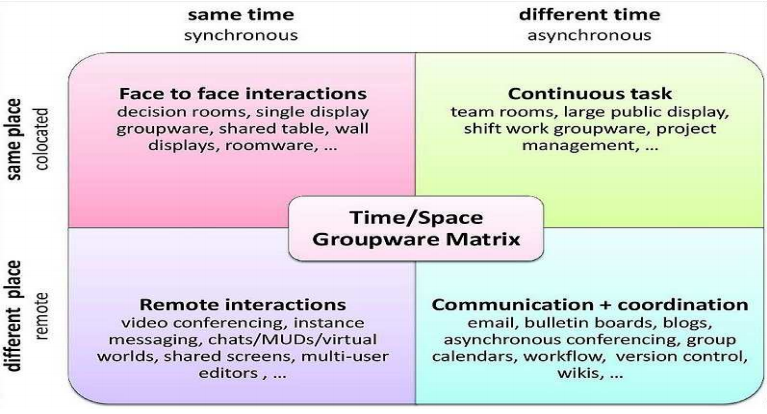
\includegraphics[scale=0.7]{chap1/images/categorizationJoh.png}
    \caption{Matrice $2\times 2$ de \textit{Johansen} pour la cat�gorisation des syst�mes de CSCW.}
	 \label{figCscwToolCateg1}
\end{figure}



\mySection{Synth�se}{}\label{sectionSyntheseChap1}
Dans...


	\myChapter{L'�dition coop�rative des documents structur�s}{}\label{chapEditionStructure}

\begin{table}
	\caption{Un tableau}
	\begin{flushleft}
	\begin{tabular}[t]{lcp{5.3cm}l}
	$\langle A,w_{1} \rangle$ & $\longrightarrow$ & $(P_{1}, [\langle C,u \rangle, \langle B,v \rangle])$ & si $w_{1}=u[v]$ \\
	
	\end{tabular}
	\begin{tabular}[t]{lcp{5.3cm}l}
	
	$\langle A,w_{2} \rangle$ & $\longrightarrow$ & $(P_{1}, [\langle C,u \rangle, \langle B,w_{11} \rangle])$ & si $w_{2}=uw_{11}$ avec $w_{11}=[_{\omega}\, ]_{\omega}$ \\
	
	\end{tabular}
	\begin{tabular}[t]{lcp{5.3cm}l}
	
	$\langle A,w_{3} \rangle$ & $\longrightarrow$ & $(P_{2}, [\,])$ & si $w_{3}=\epsilon$\\
	
	\end{tabular}
	\begin{tabular}[t]{lcp{5.3cm}l}
	
	$\langle A,w_{4} \rangle$ & $\longrightarrow$ & $(A_{\omega}, [\,])$ & si $w_{4}=(_{\omega}\, )_{\omega}$\\
	
	\end{tabular}
	\begin{tabular}[t]{lcp{5.3cm}l}
	
	$\langle B,w_{5} \rangle$ & $\longrightarrow$ & $(P_{3}, [\langle C,u \rangle, \langle A,v \rangle])$ & si $w_{5}=u(v)$ \\
	
	\end{tabular}
	\begin{tabular}[t]{lcp{5.3cm}l}
	
	$\langle B,w_{6} \rangle$ & $\longrightarrow$ & $(P_{3}, [\langle C,u \rangle, \langle A,w_{4} \rangle])$ & si $w_{6}=uw_{4}$ \\
	
	\end{tabular}
	\begin{tabular}[t]{lcp{5.3cm}l}
	
	$\langle B,w_{7} \rangle$ & $\longrightarrow$ & $(P_{4}, [\langle B,u \rangle, \langle B,v \rangle])$ & si $w_{7}=[u][v]$\\
	
	\end{tabular}
	\begin{tabular}[t]{lcp{5.3cm}l}
	
	$\langle B,w_{8} \rangle$ & $\longrightarrow$ & $(P_{4}, [\langle B,w_{11} \rangle, \langle B,v \rangle])$ & si $w_{8}=w_{11}[v]$\\
	
	\end{tabular}
	\begin{tabular}[t]{lcp{5.3cm}l}
	
	$\langle B,w_{9} \rangle$ & $\longrightarrow$ & $(P_{4}, [\langle B,u \rangle, \langle B,w_{11} \rangle])$ & si $w_{9}=[u]w_{11}$\\
	
	\end{tabular}
	\begin{tabular}[t]{lcp{5.3cm}l}
	
	$\langle B,w_{10} \rangle$ & $\longrightarrow$ & $(P_{4}, [\langle B,w_{11} \rangle, \langle B,w_{11} \rangle])$ & si $w_{10}=w_{11}w_{11}$\\
	
	\end{tabular}
	\begin{tabular}[t]{lcp{5.3cm}l}
	
	$\langle B,w_{11} \rangle$ & $\longrightarrow$ & $(B_{\omega}, [\,])$ & si $w_{11}=[_{\omega}\, ]_{\omega}$\\
	
	\end{tabular}
	\begin{tabular}[t]{lcp{5.3cm}l}
	
	$\langle C,w_{12} \rangle$ & $\longrightarrow$ & $(P_{5}, [\langle A,u \rangle, \langle C,v \rangle])$ & si $w_{12}=(u)v$ \\
	
	\end{tabular}
	\begin{tabular}[t]{lcp{5.3cm}l}
	
	$\langle C,w_{13} \rangle$ & $\longrightarrow$ & $(P_{5}, [\langle A,w_{4} \rangle, \langle C,v \rangle])$ & si $w_{13}=w_{4}v$ \\
	
	\end{tabular}
	\begin{tabular}[t]{lcp{5.3cm}l}
	
	$\langle C,w_{14} \rangle$ & $\longrightarrow$ & $(P_{6}, [\langle C,u \rangle, \langle C,v \rangle])$ & si $w_{14}=uv\neq\epsilon$\\
	
	\end{tabular}
	\begin{tabular}[t]{lcp{5.3cm}l}
	
	$\langle C,w_{15} \rangle$ & $\longrightarrow$ & $(C_\omega,[\,])$ & si $w_{15}=\epsilon$\\
	
	\end{tabular}
	\end{flushleft}
\end{table}

	\myChapter{Fusion consensuelle des mises � jour des r�pliques partielles}{}\label{chapFusionConsens}

	\myChapter{Un prototype d'�diteur coop�ratif d�synchronis� (TinyCE v2)}{}\label{chapTinyCE}

	
	%Ainsi de suite
	
	%\myChapterStar{Titre}{Titre court}{Ajouter � la table des mati�res? (false|true|chapter|section|subsection|subsubsection -chapter par d�faut-)}
\myChapterStar{Conclusion g�n�rale}{}{true}
\myMiniToc{}{Contents}

Le bilan...

%\mySectionStar{Titre}{Titre court}{Ajouter � la table des mati�res? (false|true|chapter|section|subsection|subsubsection -section par d�faut-)}
\mySectionStar{La probl�matique �tudi�e et les choix m�thodologiques}{}{true}
Nous... 

\mySectionStar{Analyse critique des r�sultats obtenus}{}{true}
Sachant...

\mySectionStar{Quelques perspectives}{}{true}
Ce travail...



\myCleanStarChapterEnd

	
	%************ Bibliographie ***************
	% La charte de l'�cole doctorale recommande un style dans lequel les citations seront de la forme (NomAuteur, Ann�e) ou (NomAuteur et al., Ann�e)
	%\myBibliography{style}{url du fichier .bib}
	\myBibliography{apalike}{bibliography}
	
	% *********** Annexes *********************
	\appendix
	
	\myChapter{Un autre exemple complet de fusion consensuelle}{Un autre exemple complet de fusion consensuelle}\label{annexeFusions}
\mySaveMarks
Dans cette annexe...

\mySectionStar{Les sch�mas des r�gles de transition}{}{false}
Rappelons que les sch�mas des transitions (compl�t�s pour prendre en compte les documents non clos) de l'automate permettant de repr�senter les expansions des r�pliques partielles suivant la vue $\mathcal{V}_1 = \{A,B\}$ lorsqu'on associe les symboles de Dyck '(' et ')' (resp. '[' et ']') au symbole visible $A$ (resp. $B$) et qu'on associe les symboles '($_{\omega}$' et ')$_{\omega}$' (resp. '[$_{\omega}$' et ']$_{\omega}$') au bourgeon $A_{\omega}$ (resp. $B_{\omega}$) de type $A$ (resp. $B$), sont les suivants:

\begin{table}
	\caption{Les sch�mas des r�gles de transition pour notre exemple}
	\begin{flushleft}
	\begin{tabular}[t]{lcp{5.3cm}l}
	$\langle A,w_{1} \rangle$ & $\longrightarrow$ & $(P_{1}, [\langle C,u \rangle, \langle B,v \rangle])$ & si $w_{1}=u[v]$ \\
	
	\end{tabular}
	\begin{tabular}[t]{lcp{5.3cm}l}
	
	$\langle A,w_{2} \rangle$ & $\longrightarrow$ & $(P_{1}, [\langle C,u \rangle, \langle B,w_{11} \rangle])$ & si $w_{2}=uw_{11}$ avec $w_{11}=[_{\omega}\, ]_{\omega}$ \\
	
	\end{tabular}
	\begin{tabular}[t]{lcp{5.3cm}l}
	
	$\langle A,w_{3} \rangle$ & $\longrightarrow$ & $(P_{2}, [\,])$ & si $w_{3}=\epsilon$\\
	
	\end{tabular}
	\begin{tabular}[t]{lcp{5.3cm}l}
	
	$\langle A,w_{4} \rangle$ & $\longrightarrow$ & $(A_{\omega}, [\,])$ & si $w_{4}=(_{\omega}\, )_{\omega}$\\
	
	\end{tabular}
	\begin{tabular}[t]{lcp{5.3cm}l}
	
	$\langle B,w_{5} \rangle$ & $\longrightarrow$ & $(P_{3}, [\langle C,u \rangle, \langle A,v \rangle])$ & si $w_{5}=u(v)$ \\
	
	\end{tabular}
	\begin{tabular}[t]{lcp{5.3cm}l}
	
	$\langle B,w_{6} \rangle$ & $\longrightarrow$ & $(P_{3}, [\langle C,u \rangle, \langle A,w_{4} \rangle])$ & si $w_{6}=uw_{4}$ \\
	
	\end{tabular}
	\begin{tabular}[t]{lcp{5.3cm}l}
	
	$\langle B,w_{7} \rangle$ & $\longrightarrow$ & $(P_{4}, [\langle B,u \rangle, \langle B,v \rangle])$ & si $w_{7}=[u][v]$\\
	
	\end{tabular}
	\begin{tabular}[t]{lcp{5.3cm}l}
	
	$\langle B,w_{8} \rangle$ & $\longrightarrow$ & $(P_{4}, [\langle B,w_{11} \rangle, \langle B,v \rangle])$ & si $w_{8}=w_{11}[v]$\\
	
	\end{tabular}
	\begin{tabular}[t]{lcp{5.3cm}l}
	
	$\langle B,w_{9} \rangle$ & $\longrightarrow$ & $(P_{4}, [\langle B,u \rangle, \langle B,w_{11} \rangle])$ & si $w_{9}=[u]w_{11}$\\
	
	\end{tabular}
	\begin{tabular}[t]{lcp{5.3cm}l}
	
	$\langle B,w_{10} \rangle$ & $\longrightarrow$ & $(P_{4}, [\langle B,w_{11} \rangle, \langle B,w_{11} \rangle])$ & si $w_{10}=w_{11}w_{11}$\\
	
	\end{tabular}
	\begin{tabular}[t]{lcp{5.3cm}l}
	
	$\langle B,w_{11} \rangle$ & $\longrightarrow$ & $(B_{\omega}, [\,])$ & si $w_{11}=[_{\omega}\, ]_{\omega}$\\
	
	\end{tabular}
	\begin{tabular}[t]{lcp{5.3cm}l}
	
	$\langle C,w_{12} \rangle$ & $\longrightarrow$ & $(P_{5}, [\langle A,u \rangle, \langle C,v \rangle])$ & si $w_{12}=(u)v$ \\
	
	\end{tabular}
	\begin{tabular}[t]{lcp{5.3cm}l}
	
	$\langle C,w_{13} \rangle$ & $\longrightarrow$ & $(P_{5}, [\langle A,w_{4} \rangle, \langle C,v \rangle])$ & si $w_{13}=w_{4}v$ \\
	
	\end{tabular}
	\begin{tabular}[t]{lcp{5.3cm}l}
	
	$\langle C,w_{14} \rangle$ & $\longrightarrow$ & $(P_{6}, [\langle C,u \rangle, \langle C,v \rangle])$ & si $w_{14}=uv\neq\epsilon$\\
	
	\end{tabular}
	\begin{tabular}[t]{lcp{5.3cm}l}
	
	$\langle C,w_{15} \rangle$ & $\longrightarrow$ & $(C_\omega,[\,])$ & si $w_{15}=\epsilon$\\
	
	\end{tabular}
	\end{flushleft}
\end{table}

De m�me...



\myRestoreMarks

	\myChapter{Quelques fonctions Haskell pour le calcul des consensus}{}\label{annexeFonctionsHask}
\mySaveMarks
Dans cette annexe...

\mySectionStar{Repr�sentation des grammaires et des vues}{}{false}
Une grammaire est constitu�e d'un ensemble de symboles et d'un ensemble de productions. Nous repr�sentons une grammaire par le type \Verb|Gram| suivant:
\begin{Verbatim}[fontsize=\small, numbers=left, numbersep=8pt]
data Gram prod symb = Gram {prods::[prod], 
                            symbols::[symb], 
                            lhs::prod -> symb, 
                            rhs::prod -> [symb]}
\end{Verbatim}

La fonction \Verb|lhs| (resp. \Verb|rhs|) prend en argument une grammaire \Verb|G| et une production \Verb|p| de \Verb|G| puis retourne le symbole en partie gauche (resp. la liste des symboles en partie droite) de \Verb|p|. \`{A} partir de ce type, on peut construire la grammaire $\mathbb{G}_{expl}$ (chap \ref{chapEditionStructure} exemple \ref{exempleGrammaire}) gr�ce au code Haskell suivant:
\begin{Verbatim}[fontsize=\small, numbers=left, numbersep=8pt]
data Prod = P1 | P2 | P3 | P4 | P5 | P6 | P7 | Aomega | Bomega | Comega
            deriving (Eq, Show)
data Symb = A | B | C  deriving (Eq, Show)

gram :: Gram Prod Symb
gram = Gram lprod lsymb lhs_ rhs_
   where
      lprod = [P1, P2, P3, P4, P5, P6, P7]
      lsymb = [A, B, C]
      lhs_ p = case p of
            P1 -> A; P2 -> A; P3 -> B; P4 -> B; P5 -> C; P6 -> C; P7 -> C
      rhs_ p = case p of
            P1 -> [C, B]; P2 -> []; P3 -> [C, A]; P4 -> [B, B]; 
            P5 -> [A, C]; P6 -> [C, C]; P7 -> []
\end{Verbatim}

Les productions \Verb|Aomega, Bomega| et \Verb|Comega| ont �t� introduites pour pouvoir d�signer les bourgeons de types respectifs \Verb|A|, \Verb|B| et \Verb|C|.


\myRestoreMarks

	%Ainsi de suite
}
\end{document}
